\chapter{可換な観測量、エネルギー位相、スピン歳差}

\lectureoverview{まず不確定性の定性的な意味から始める。二つの観測量が同時に確定値をもちうるのは、完全な共通固有基底をもつ場合に限られ、これはそれらの演算子が可換であることと等価である。次にユニタリ発展とSchr\"odinger方程式を復習し、交換子を古典的なポアソン括弧と比較し、エネルギー基底で時間依存方程式を解き、その結果を磁場中のスピンに適用する。最後の計算から、スピン期待値の歳差運動、一般のスピンハミルトニアンの二つのエネルギー準位、および横向きの期待値とエネルギーギャップの半分のエネルギーの光子との区別が得られる。}

二状態スピンは依然として最も単純な量子系である。三状態ヒルベルト空間が次に単純な抽象的候補であろうが、二つのスピンはすでに四つの直交基底状態をもつ。二つのスピンをまだ合成することはしないが、その段階は近く、そこにはもつれが伴う。まず一つのスピンの問題を片付け、不確定性と時間発展の考え方をより確かな基盤の上に置くべきである。

\section{二つの量が同時に確定値をもちうる場合}

良い測定は繰り返し可能である。ある観測量を測定して値\(l\)が得られたなら、直ちに繰り返せば同じ値が返るはずである。したがって最初の測定は、少なくともその瞬間、系を対応する演算子の固有状態に残さなければならない：
\begin{equation}
L\ket{l}=l\ket{l}.
\end{equation}
この操作的な記述だけで、不確定性の定性的な起源を明らかにするのに十分である。

二つの観測量\(L\)と\(M\)が同時に測定できるとしよう。同時測定は報告される両方の値を確定に保たなければならない。したがってその測定後の可能な状態は、両方の演算子の同時固有ベクトルでなければならない。ここで用いる有限次元の設定では、次を満たす完全な正規直交集合\(\{\ket{i}\}\)を選べる：
\begin{equation}
L\ket{i}=l_i\ket{i},
\qquad
M\ket{i}=m_i\ket{i}.
\label{eq:l5-common-eigenvectors}
\end{equation}

\begin{remark}ここで\emph{基底}という語は完全な正規直交基底を意味する。線形代数は非直交基底も許すが、正規直交という約束は量子状態にとって特に自然である。縮退した固有値は固有空間内に自由度を残すが、その空間内では固有ベクトルを正規直交に選べる。
\end{remark}

\begin{theorem}二つの有限次元エルミート観測量が同時に測定可能であるのは、それらが完全な共通固有基底をもつとき、等価にいえば可換であるときに、まさにそのときに限る。
\end{theorem}

順方向は式~\eqref{eq:l5-common-eigenvectors}から直ちに従う。一方の順序で作用させると
\begin{align}
ML\ket{i}
&=M\bigl(l_i\ket{i}\bigr)\\
&=l_i m_i\ket{i},
\end{align}
となり、逆の順序では
\begin{align}
LM\ket{i}
&=L\bigl(m_i\ket{i}\bigr)\\
&=m_i l_i\ket{i}.
\end{align}
となる。固有値は通常の数であるから\(l_i m_i=m_i l_i\)である。したがって\(ML\)と\(LM\)は基底の各要素に、ひいては任意の状態に同一に作用する：
\begin{equation}
[L,M]\equiv LM-ML=0.
\label{eq:l5-commuting-condition}
\end{equation}

\begin{figure}[htbp]
\centering
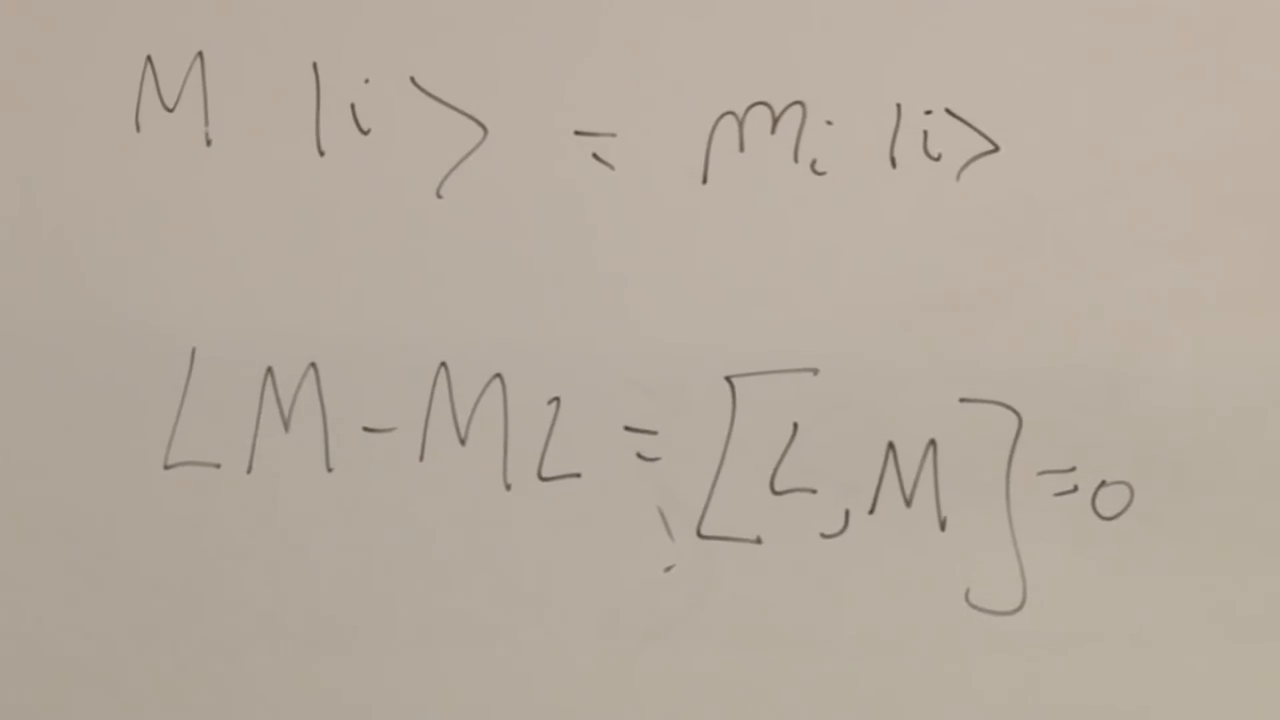
\includegraphics[width=0.86\textwidth]{lecture_05_figure_02.png}
\caption{共通固有ベクトルの議論は\(LM-ML=[L,M]=0\)に到達する。}
\lectureframe{00:10:30}
\end{figure}

逆もまた真である：可換なエルミート演算子は同時に対角化できる。一方の演算子が縮退した固有空間をもつなら、他方はその固有空間を保ち、その中で対角化できる。これを各固有空間で繰り返せば、完全な共通固有基底が得られる。

パウリ演算子が最初の重要な反例を与える。\(\sigma_x,\sigma_y,\sigma_z\)のうちどの二つも可換でない。\(\sigma_z\)の固有状態は上と下であり、\(\sigma_x\)の固有状態は右と左である。どちらか一方の成分を鋭く準備してその測定を繰り返すことはできるが、両方の成分を同時に鋭く準備することはできない。これは数値的な不等式が導入される前の不確定性である。

後に、非可換な二つの観測量の不確定性が互いをどのように制約するかを定量化する。ここで数値的な不確定性原理を証明しているのではない。現在の要点は不等式より前にある：非可換性は、一つの状態が両方の量に同時に確定値を割り当てることを妨げる。

\begin{classroomqa}
\audiencequestion{なぜ同時測定には共通固有ベクトルが必要なのか。}
\lecturerresponse{繰り返し可能な測定は、測定値が確定した状態、すなわち測定された演算子の固有状態を残す。二つの値が同時に得られ、両方が繰り返し可能であり続けるなら、結果として得られる状態は両方の演算子の固有状態でなければならない。したがって同時結果の完全な集合が共通固有基底を与える。}
\end{classroomqa}

\begin{classroomqa}
\audiencequestion{これは二つの異なる粒子に関わるのか。}
\lecturerresponse{必ずしもそうではない。\(\sigma_x\)と\(\sigma_z\)はすでに一つのスピンに作用するからである。しかし二つの異なる部分系については、異なる因子に作用する観測量は可換である：\(A\otimes I\)は\(I\otimes B\)と可換である。だからこそ一方のスピンの成分と他方のスピンの成分を同時に測定できる。このような系を合成することは後に量子もつれへと導く。}
\end{classroomqa}

\section{ユニタリ発展とその生成子}

量子力学が状態を定義するのに要した時間は古典力学よりかなり長かったが、状態空間さえ確立されれば、運動の規則は簡潔である。
\begin{equation}
\ket{\psi(t)}=U(t)\ket{\psi(0)}.
\label{eq:l5-propagator}
\end{equation}
時間発展は識別可能性を保たなければならない。さらに強く、すべての内積を保つ。正規直交基底に対して
\begin{equation}
\bra{j}U^\dagger(t)U(t)\ket{i}=\delta_{ji},
\end{equation}
したがって
\begin{equation}
U^\dagger(t)U(t)=I.
\label{eq:l5-unitarity}
\end{equation}
発展演算子はユニタリである。

経過時間がゼロのとき \(U(0)=I\)。連続性により、微小時間 \(\epsilon\) の発展は恒等演算子とわずかしか異ならない。\(\hbar=1\) の単位で
\begin{equation}
U(\epsilon)=I-i\epsilon H+O(\epsilon^2),
\qquad
U^\dagger(\epsilon)=I+i\epsilon H^\dagger+O(\epsilon^2).
\end{equation}
と書く。式~\eqref{eq:l5-unitarity}に代入すると
\begin{equation}
H^\dagger=H.
\end{equation}
時間発展の生成子はエルミートであり、したがって観測量である。それがハミルトニアンである。

微小伝播子を状態に適用すると
\begin{equation}
\ket{\psi(\epsilon)}
=\ket{\psi(0)}-i\epsilon H\ket{\psi(0)}+O(\epsilon^2).
\end{equation}
となる。整理すると、黒板に示された差分商が得られる：
\begin{equation}
\frac{\ket{\psi(\epsilon)}-\ket{\psi(0)}}{\epsilon}
=-iH\ket{\psi(0)}+O(\epsilon).
\end{equation}

\begin{figure}[htbp]
\centering
\includegraphics[width=0.86\textwidth]{lecture_05_figure_03.png}
\caption{差分商として書かれた微小更新。}
\lectureframe{00:23:33}
\end{figure}

\(\epsilon\to0\) とすると、時間依存の Schr\"odinger 方程式が得られる：
\begin{equation}
\frac{d}{dt}\ket{\psi(t)}=-iH\ket{\psi(t)}.
\label{eq:l5-schrodinger}
\end{equation}
定数を復元すれば、これは \(i\hbar\,d\ket{\psi}/dt=H\ket{\psi}\) である。

Schr\"odinger の元の方程式は運動する粒子の波動関数に関するものであった。上記の演算子による定式化は、スピン、三状態系、二つのスピン、あるいは任意の複雑さの系にも等しく適用されるため、かつて一般化された Schr\"odinger 方程式と呼ばれた。その形容詞はほとんど使われなくなり、今では単に方程式の一般形である。

式~\eqref{eq:l5-schrodinger}は、系が乱されずに放置されるときの状態の確定した発展を与える。これはすべての実験結果が確定することを意味しない。量子状態は可能な測定に対する確率を定め、方程式は変化する振幅を通じてそれらの確率を更新する。測定は一般に状態を変え、この孤立した発展を中断する。

\begin{classroomqa}
\audiencequestion{すべての測定は系を乱すのか？}
\lecturerresponse{一般には、そうである。しかし重要な特別な場合がある。状態がすでに観測量の固有状態であれば、理想的で繰り返し可能な測定はその状態を変えずに値を確認できる。一般に成り立たないのは、他の非可換な性質を乱さずに任意の観測量を測定できる可能性である。}
\end{classroomqa}

\section{エネルギーと時間に依存しない方程式}

\(H\) はエルミートであるから、その固有値は実数であり、固有ベクトルは完全な正規直交基底として選べる：
\begin{equation}
H\ket{E_i}=E_i\ket{E_i}.
\label{eq:l5-time-independent}
\end{equation}
これは Schr\"odinger 方程式の時間に依存しない形である。運動方程式ではなく固有値問題であり、系がどのようなエネルギー値をもち得るか、またどの状態がそれらの値をもつかを問う。

スペクトルは系に依存する。束縛された原子運動や調和振動子は可算個のエネルギー準位をもつ。束縛されていない粒子は連続スペクトルをもち得る。エネルギーは多くの方法で測定できる。原理的には、十分に精密な質量測定でも \(E=mc^2\) を用いうるが、実際の方法としてはほとんど用いられない。実在の系はすでにそのハミルトニアンをもっており、物理学者はそれを指示するのではなく、発見しようとする。その演算子がわかれば、その固有値と固有ベクトルを求めることが数学的課題である。

\(H\) に定数 \(cI\) を加えると、すべてのエネルギーが \(c\) だけずれる。それは状態全体を共通の位相 \(e^{-ict}\) 倍するだけで、確率や期待値を変えない。ここで考える力学に影響するのはエネルギー差だけである。

\section{期待値はどのように動くか}

標準的な表現 \emph{期待値} は統計的平均を意味する。観測量 \(L\) に対して
\begin{equation}
\expect{L}(t)=\bra{\psi(t)}L\ket{\psi(t)}.
\end{equation}
この段階では状態ベクトルだけが時間依存性をもつ。両辺を微分し、式~\eqref{eq:l5-schrodinger}とそのエルミート共役を用いると
\begin{equation}
\frac{d}{dt}\ket{\psi}=-iH\ket{\psi},
\qquad
\frac{d}{dt}\bra{\psi}=i\bra{\psi}H,
\end{equation}
から
\begin{align}
\frac{d}{dt}\expect{L}
&=i\bra{\psi}HL\ket{\psi}
  -i\bra{\psi}LH\ket{\psi}\\
&=-i\expect{[L,H]}.
\label{eq:l5-expectation-motion}
\end{align}
が得られる。

\begin{figure}[htbp]
\centering
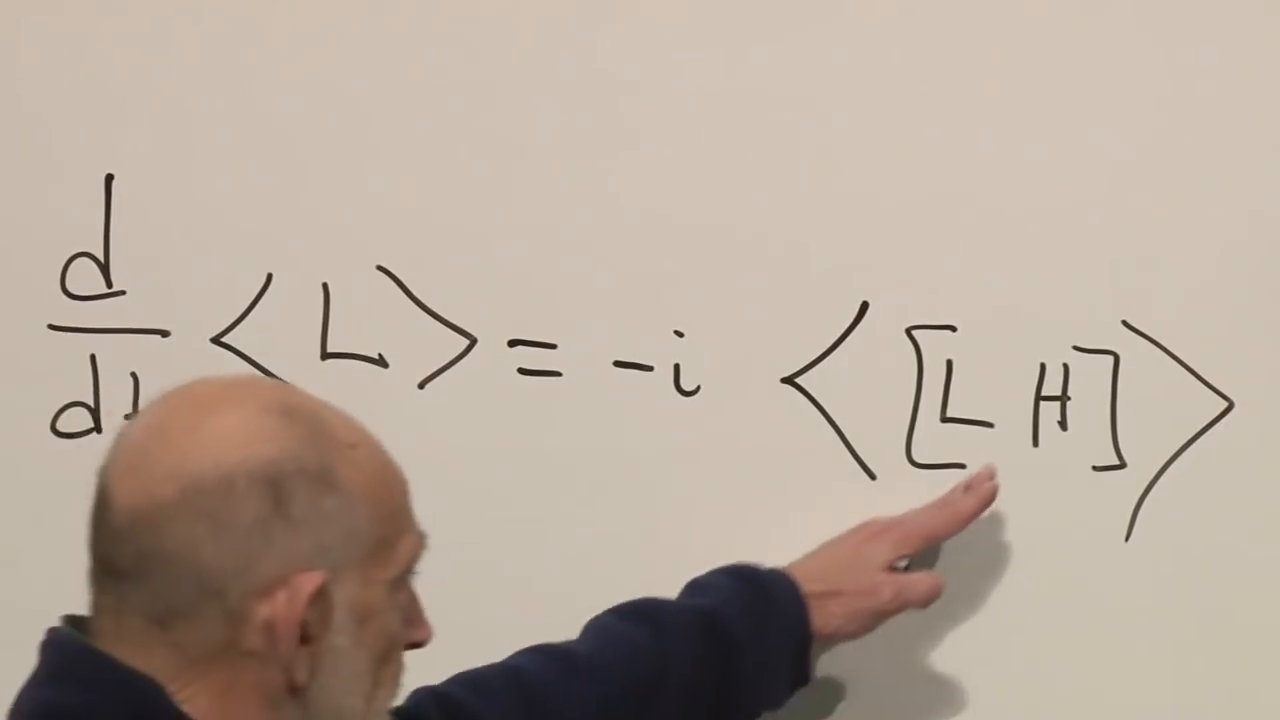
\includegraphics[width=0.86\textwidth]{lecture_05_figure_04.png}
\caption{交換子の形で書かれた期待値の運動方程式。}
\lectureframe{00:35:35}
\end{figure}

因子 \(i\) は \(\expect{L}\) の実在性を脅かすものではない。エルミートな \(L\) と \(H\) に対して、交換子は反エルミートである：
\begin{equation}
[L,H]^\dagger=-[L,H].
\end{equation}
したがってその期待値は純虚数であり、\(-i\) を掛けると実数の導関数が得られる。

しばしば次の略記が書かれる：
\begin{equation}
\dot L=-i[L,H].
\end{equation}
現時点では、これは式~\eqref{eq:l5-expectation-motion}の略記、すなわち平均に関する方程式として読むべきである。演算子自身が時間依存性をもつ完全な描像の変更は後で現れる。

\subsection{交換子の代数}

交換子は反対称である：
\begin{equation}
[A,B]=-[B,A].
\end{equation}
また、微分に対するライプニッツ則に類似した積の規則に従う：
\begin{equation}
[AB,C]=A[B,C]+[A,C]B.
\label{eq:l5-product-rule}
\end{equation}
これを検証するには、すべての因子の順序を保つ：
\begin{align}
A[B,C]+[A,C]B
&=A(BC-CB)\\
&\quad +(AC-CA)B\\
&=ABC-ACB\\
&\quad +ACB-CAB\\
&=ABC-CAB\\
&=[AB,C].
\end{align}

\begin{figure}[htbp]
\centering
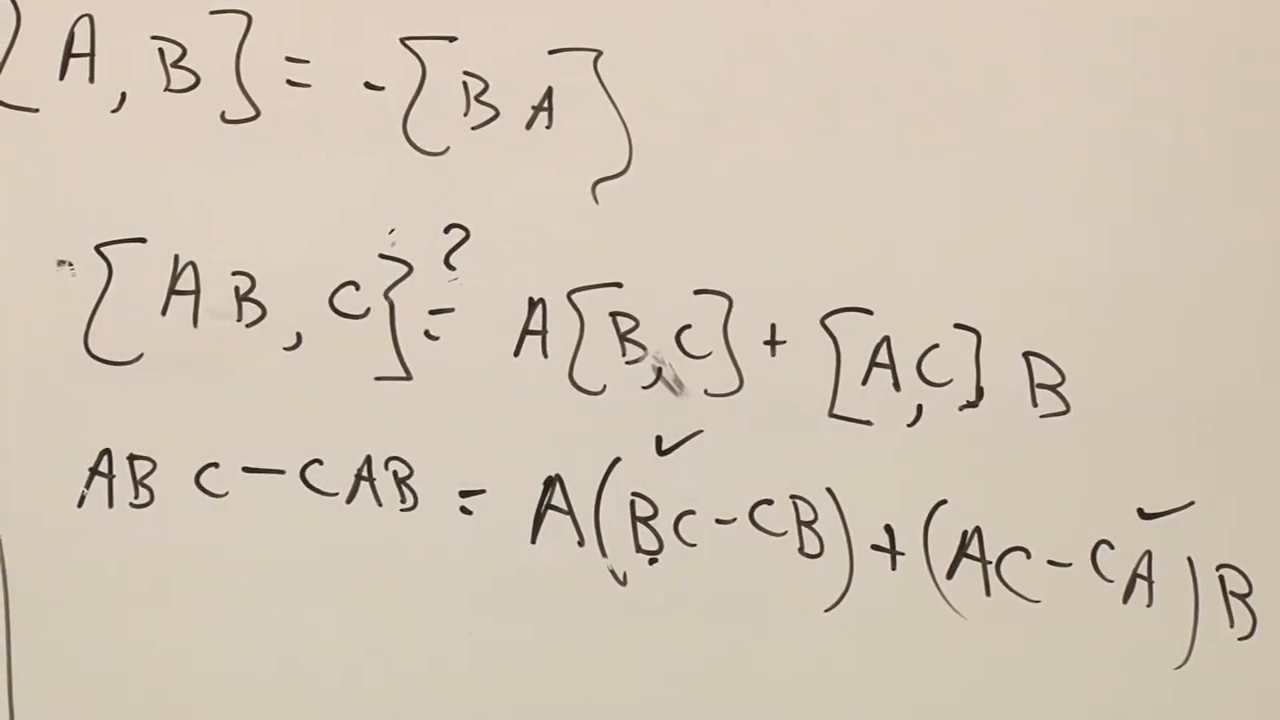
\includegraphics[width=0.86\textwidth]{lecture_05_figure_05.png}
\caption{両辺を展開して確認した交換子の積の規則。}
\lectureframe{00:43:10}
\end{figure}

\begin{classroomqa}
\audiencequestion{積の規則の右辺は、誤って左辺を二重に数えていないか？}
\lecturerresponse{いいえ。展開すると、\(ABC\) と \(-CAB\) が求める二つの項である。挿入された二つの項は \(-ACB\) と \(+ACB\) であり、これらは正確に相殺する。余分に見える複製は、要求される二通りの方法で式を因数分解するために必要な一時的な項である。}
\end{classroomqa}

同じ反対称性と積の規則が古典的ポアソン括弧にも成り立つ。この構造的類似は偶然ではない。古典的対応は
\begin{equation}
\{A,B\}
\quad\longleftrightarrow\quad
\frac{1}{i\hbar}[A,B]
=-\frac{i}{\hbar}[A,B].
\label{eq:l5-poisson-correspondence}
\end{equation}
\(\hbar=1\) 単位では、古典的方程式
\begin{equation}
\frac{dL}{dt}=\{L,H\}
\end{equation}
は式~\eqref{eq:l5-expectation-motion}と同じ形をとる。通常の巨視的単位では \(\hbar\) は微小であり、適切な古典極限で交換子は無視できるようになる。これが、量子的生成子 \(H\) を古典力学のハミルトニアンと同一視する本質的な検証である。

\(\hbar\) の因子は次元の要請から必要である。ポアソン括弧は共役な座標と運動量に関して微分するのに対し、演算子の交換子は積から直接構成される。プランク定数がこれらの次元の間の換算を与える。

\(L=H\) と置く。すべての演算子はそれ自身と可換であるから、
\begin{equation}
\frac{d}{dt}\expect{H}
=-i\expect{[H,H]}=0.
\end{equation}
ここで議論している時間に依存しないハミルトニアンに対して、平均エネルギーは保存される。完全なエネルギー分布についてより強い主張も可能であるが、ここで必要なのは平均だけである。

\begin{classroomqa}
\audiencequestion{これらの方程式における \(L\) とは何か？角運動量か？}
\lecturerresponse{ここで \(L\) は一般的なエルミート線形演算子であり、したがって任意の観測量である。スピン成分、位置、あるいは \(H\) 自身であってもよい。この文字は \emph{線形演算子} に対して選ばれたものであり、その意味が別途述べられていない限り角運動量と読むべきではない。}
\end{classroomqa}

\begin{classroomqa}
\audiencequestion{なぜ因子 \(i\) は、実の平均値に虚の導関数を生じさせないのか？}
\lecturerresponse{二つのエルミート演算子の交換子は反エルミートであるから、その期待値は虚である。以下のパウリ行列の計算がこれを具体的にする：それらの交換子は明示的な因子 \(2i\) を含み、これが運動方程式の \(-i\) を相殺する。}
\end{classroomqa}

\section{エネルギー基底における Schr\"odinger 方程式の求解}

エネルギー固有値問題が解かれていると仮定する。任意の状態を固定されたエネルギー基底で展開する：
\begin{equation}
\ket{\psi(t)}=\sum_j\alpha_j(t)\ket{E_j}.
\label{eq:l5-energy-expansion}
\end{equation}
この記述では基底ベクトルは変化せず、すべての時間依存性は係数にある。式~\eqref{eq:l5-energy-expansion}を式~\eqref{eq:l5-schrodinger}に代入すると
\begin{align}
\sum_j\dot\alpha_j(t)\ket{E_j}
&=-i\sum_j\alpha_j(t)H\ket{E_j}\\
&=-i\sum_j E_j\alpha_j(t)\ket{E_j}.
\end{align}
基底における展開の一意性から、各固定された \(j\) に対して
\begin{equation}
\dot\alpha_j(t)=-iE_j\alpha_j(t),
\qquad\text{no sum on \(j\)}.
\end{equation}
解は
\begin{equation}
\alpha_j(t)=\alpha_j(0)e^{-iE_jt}.
\label{eq:l5-energy-phase}
\end{equation}

\begin{figure}[htbp]
\centering
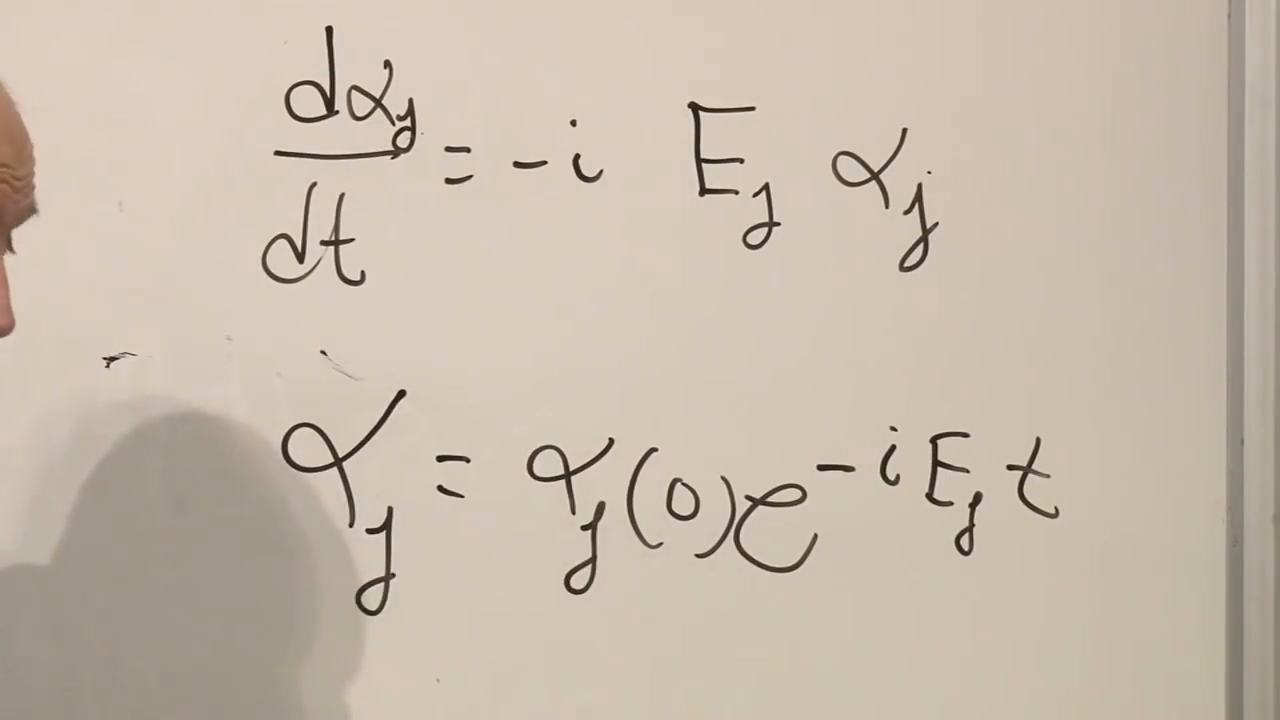
\includegraphics[width=0.86\textwidth]{lecture_05_figure_06.png}
\caption{各エネルギー基底係数はそれ自身の指数位相方程式を満たす。}
\lectureframe{01:03:25}
\end{figure}

したがって一般解は
\begin{equation}
\ket{\psi(t)}
=\sum_j\alpha_j(0)e^{-iE_jt}\ket{E_j}.
\label{eq:l5-general-solution}
\end{equation}
単位を戻すと \(E_jt\) が \(E_jt/\hbar\) に置き換わる。すべての係数の大きさは固定されたままである：
\begin{equation}
|\alpha_j(t)|=|\alpha_j(0)|.
\end{equation}
時間発展は相対位相を変化させる。単一のエネルギー固有状態は一つの共通位相だけを獲得し、したがって時間に依存しない測定確率をもつ。

\(L\) の期待値は今や明示的に書ける。エネルギー基底におけるその行列要素を
\begin{equation}
L_{kj}=\bra{E_k}L\ket{E_j}.
\end{equation}
で定義すると、
\begin{align}
\expect{L}(t)
&=\sum_{k,j}
\alpha_k^*(0)\alpha_j(0)
e^{i(E_k-E_j)t}
L_{kj}.
\label{eq:l5-heisenberg-matrix}
\end{align}

\begin{figure}[htbp]
\centering
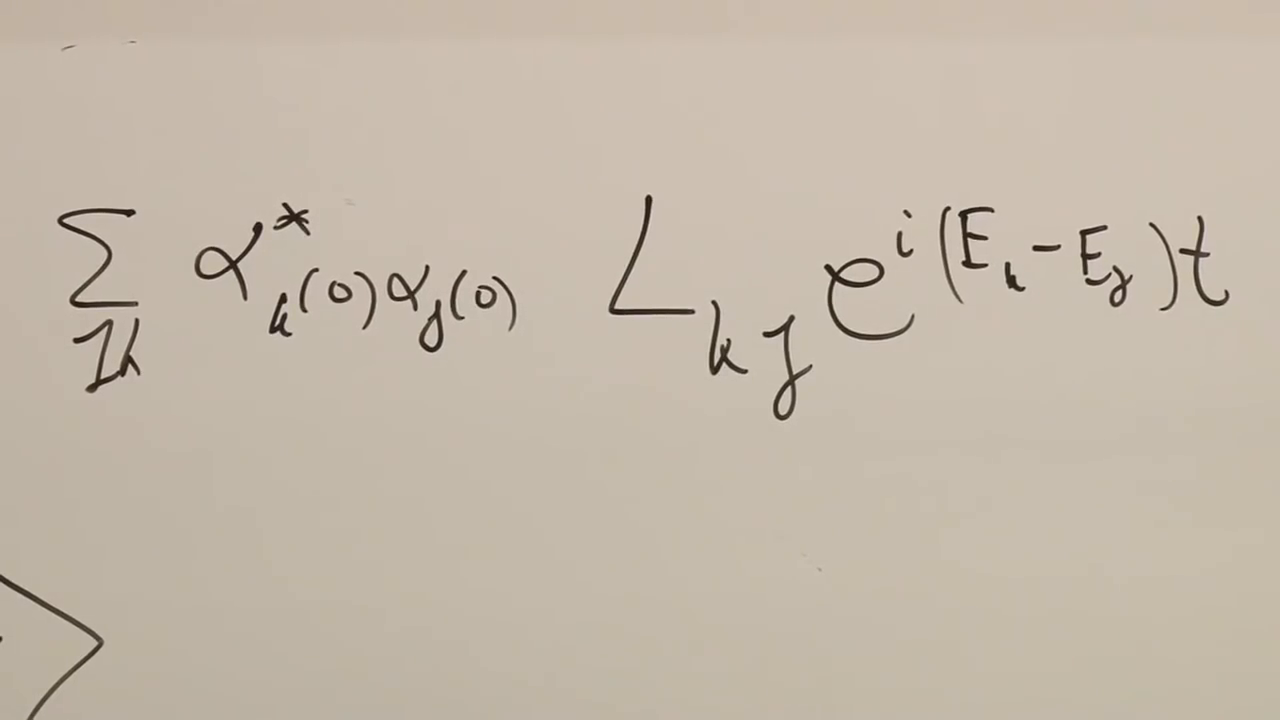
\includegraphics[width=0.86\textwidth]{lecture_05_figure_07.png}
\caption{エネルギー基底の行列公式：各要素は遷移振動数の位相を伴う。}
\lectureframe{01:10:45}
\end{figure}

対角項 \(k=j\) は定数である。非対角行列要素はエネルギー差 \(E_k-E_j\) で振動する。ここで述べた歴史的説明では、ハイゼンベルクは現代の状態ベクトルによる導出が利用可能になる前にこの行列的組織化を認識していた；ディラックの記法は後にその意味を透明にした。

\begin{classroomqa}
\audiencequestion{\(\alpha_j\) 係数の大きさは固定されたままか？}
\lecturerresponse{はい。各係数は大きさ1の複素位相を掛けられる。変化するのは相対位相だけであり、それらの位相が非対角行列要素を含む期待値を時間とともに変化させるのである。}
\end{classroomqa}

\begin{classroomqa}
\audiencequestion{Schr\"odinger方程式では偏微分と全微分のどちらを使うべきか。}
\lecturerresponse{ここで用いている抽象状態\(\ket{\psi(t)}\)では、時間が唯一の表示された変数であるため、どちらの記法でも同じ内容を表す。後に\(\psi(x,t)\)のような波動関数は位置と時間の両方に依存し、そのときには偏微分の記法が自然になる。}
\end{classroomqa}

\begin{classroomqa}
\audiencequestion{直交性の保存は単なる経験的な仮定にすぎないのか。}
\lecturerresponse{それは実験によって支持されているが、同時に異常に硬い性質でもある。ユニタリな量子力学を変形しようとする試みは、正値性や確率の保存、因果的な局所性、あるいは複合系の一貫した取り扱いを破壊しがちである。David Finkelsteinは、変形可能な理論は塑性流動を起こし、硬い理論は脆性破壊を起こすと述べた。この意味で量子力学は脆い。小さな恣意的変更によって、通常は近傍に一貫した理論が残ることはない。}
\end{classroomqa}

\begin{classroomqa}
\audiencequestion{なぜエネルギー固有値\(E_j\)は実数なのか。}
\lecturerresponse{ユニタリ性は無限小生成子\(H\)がエルミートであることを意味し、エルミート演算子のすべての固有値は実数である。したがって、その連鎖は直交性の保存、ユニタリ性、\(H\)のエルミート性、そしてエネルギー・スペクトルの実数性である。}
\end{classroomqa}

\section{磁場中のスピン}

1つのスピンにはどのようなハミルトニアンを割り当てるべきか。それ以外は空の空間にある孤立したスピンには、非自明な優先方向が存在しないため、そのハミルトニアンは単位行列に比例し、観測可能な運動を生じない。磁場は相互作用エネルギーと軸の両方を与える。

磁場を\(z\)方向にとる。スピンをもつ荷電粒子は磁気モーメントを担い、よく知られた双極子エネルギーはそのモーメントが磁場とどれだけ揃っているかに比例する。磁場の強さ、磁気モーメント、符号の規約、および\(\hbar\)を1つの定数\(\omega\)に吸収する。
\begin{equation}
H=\frac{\omega}{2}\sigma_z.
\label{eq:l5-z-hamiltonian}
\end{equation}
\(1/2\)の因子は、パウリ交換子が\(2\)の因子を含むため便利である。

古典的な矢印の描像は注意して扱わなければならない。量子スピンは\(x\)、\(y\)、\(z\)の各成分を同時に確定値として持つことはないため、通常の矢印でその性質のすべてを一度に表すことはできない。有用な三次元の対象は期待値のベクトルであり、2成分の状態ベクトルそのものではない。

\subsection{パウリ交換子}

行列表示
\begin{equation}
\begin{aligned}
\sigma_x&=
\begin{pmatrix}0&1\\1&0\end{pmatrix},\\[0.4em]
\sigma_y&=
\begin{pmatrix}0&-i\\i&0\end{pmatrix},\\[0.4em]
\sigma_z&=
\begin{pmatrix}1&0\\0&-1\end{pmatrix}.
\end{aligned}
\end{equation}
を用いる。例えば、
\begin{align}
[\sigma_z,\sigma_x]
&=
\begin{pmatrix}1&0\\0&-1\end{pmatrix}
\begin{pmatrix}0&1\\1&0\end{pmatrix}
-
\begin{pmatrix}0&1\\1&0\end{pmatrix}
\begin{pmatrix}1&0\\0&-1\end{pmatrix}\\
&=
\begin{pmatrix}0&1\\-1&0\end{pmatrix}
-
\begin{pmatrix}0&-1\\1&0\end{pmatrix}\\
&=2
\begin{pmatrix}0&1\\-1&0\end{pmatrix}
=2i\sigma_y.
\end{align}
巡回関係は
\begin{equation}
\begin{aligned}
[\sigma_z,\sigma_x]&=2i\sigma_y,\\
[\sigma_x,\sigma_y]&=2i\sigma_z,\\
[\sigma_y,\sigma_z]&=2i\sigma_x.
\end{aligned}
\label{eq:l5-pauli-commutators}
\end{equation}
であり、どちらかの添字を入れ替えると符号が反転する。

\begin{figure}[htbp]
\centering
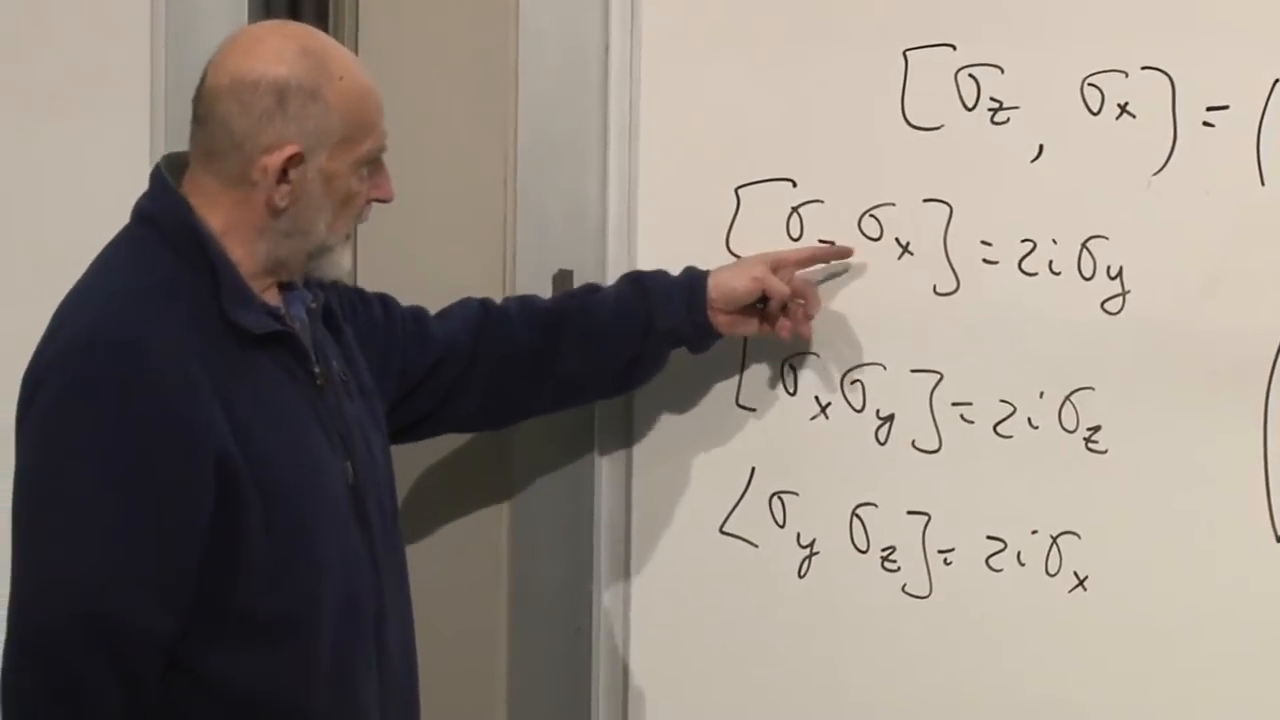
\includegraphics[width=0.86\textwidth]{lecture_05_figure_08.png}
\caption{3つのパウリ交換子は、パウリ行列自身の上で巡回的に閉じている。}
\lectureframe{01:33:30}
\end{figure}

これらの関係は、角運動量の古典的ポアソン括弧と同じ巡回構造をもつ。また、元の3つの演算子の上で閉じているため、運動方程式が特に簡単になる。

\begin{classroomqa}
\audiencequestion{交換子はブラケットを用いて計算しなければならないのか。}
\lecturerresponse{いいえ。演算子の積は行列の積で表されるため、\(2\times2\)行列が便利な直接計算を与える。代わりに演算子をアップとダウンの基底状態に順に作用させても同じ結果が得られる。}
\end{classroomqa}

\subsection{期待値の歳差運動}

式~\eqref{eq:l5-expectation-motion}を式~\eqref{eq:l5-z-hamiltonian}のハミルトニアンとともに適用すると、
\begin{align}
\frac{d}{dt}\expect{\sigma_x}
&=-i\frac{\omega}{2}\expect{[\sigma_x,\sigma_z]}
=-\omega\expect{\sigma_y},\\
\frac{d}{dt}\expect{\sigma_y}
&=-i\frac{\omega}{2}\expect{[\sigma_y,\sigma_z]}
=+\omega\expect{\sigma_x},\\
\frac{d}{dt}\expect{\sigma_z}
&=-i\frac{\omega}{2}\expect{[\sigma_z,\sigma_z]}
=0.
\label{eq:l5-spin-motion}
\end{align}

\begin{figure}[htbp]
\centering
\begin{minipage}[c]{0.62\textwidth}
\centering
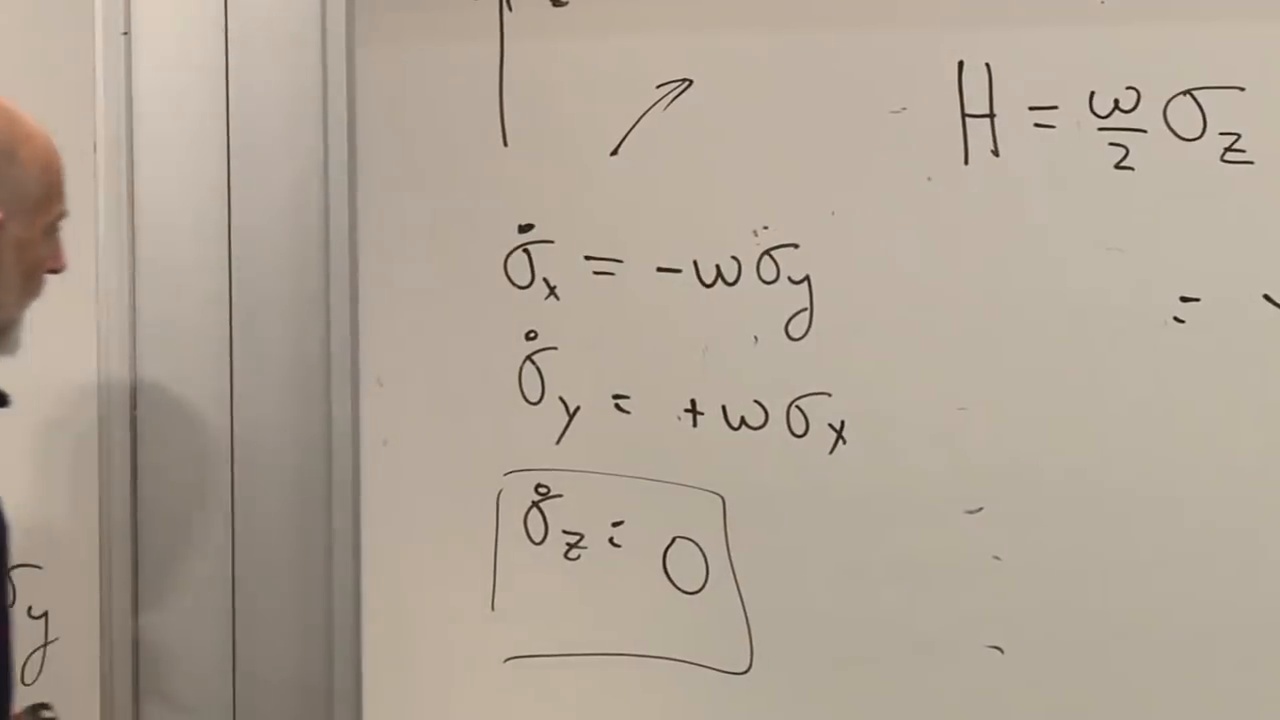
\includegraphics[width=\textwidth]{lecture_05_figure_09.png}
\end{minipage}\hfill
\begin{minipage}[c]{0.31\textwidth}
\centering
\begin{tikzpicture}[scale=0.78,>=Latex]
  \draw[->,thick] (0,0) -- (0,3.0) node[above] {\(z\parallel\bm B\)};
  \draw[dashed] (0,1.8) ellipse (1.45 and 0.42);
  \draw[->,very thick] (0,0) -- (1.05,1.8)
    node[right] {\(\expect{\bm\sigma}\)};
  \draw[->,thick] (1.38,1.67)
    arc[start angle=-12,end angle=245,x radius=1.45,y radius=0.42];
\end{tikzpicture}
\end{minipage}
\caption{黒板の式とその幾何学的帰結。横方向の平均は回転し、磁場に平行な成分は固定されたままである。矢印は3つの期待値を描いており、隠れた古典的スピンではない。}
\lectureframe{01:35:28}
\end{figure}

最初の2つの式は横平面内の円運動を記述する。
\begin{align}
\expect{\sigma_x}(t)
&=\expect{\sigma_x}(0)\cos\omega t
-\expect{\sigma_y}(0)\sin\omega t,\\
\expect{\sigma_y}(t)
&=\expect{\sigma_x}(0)\sin\omega t
+\expect{\sigma_y}(0)\cos\omega t.
\end{align}
一方、\(\expect{\sigma_z}\)は一定である。したがって期待値ベクトルは、角振動数\(\omega\)で磁場軸のまわりを歳差運動する。

このSchr\"odinger描像における演算子は固定された行列である。変化するのは状態であり、したがってよく知られたジャイロスコープ的な運動を行うのは平均値である。

\begin{classroomqa}
\audiencequestion{2次元の状態空間から、どのようにして3次元の歳差運動の描像が生じるのか。}
\lecturerresponse{状態ベクトルは、規格化と全位相を除いて2つの複素成分をもつ。それに対して描かれる実空間のベクトルは\(\bigl(\expect{\sigma_x},\expect{\sigma_y},\expect{\sigma_z}\bigr)\)である。これらの期待値は状態によって決まり、ブロッホ・ベクトルの描像を形成するが、状態ベクトルそのものではない。}
\end{classroomqa}

\section{最も一般的な1スピンのハミルトニアン}

任意のエルミートな\(2\times2\)行列は
\begin{equation}
H=aI+b_x\sigma_x+b_y\sigma_y+b_z\sigma_z,
\end{equation}
と実係数で展開できる。単位行列の項は全体の位相のみを変える。残りの3つの係数はベクトルの成分とみなせる。その大きさを\(\omega/2\)、向きを単位ベクトル\(\bm n\)と書くと、非自明なハミルトニアンは
\begin{equation}
H=\frac{\omega}{2}\,\bm\sigma\cdot\bm n,
\qquad
\bm\sigma\cdot\bm n
=n_x\sigma_x+n_y\sigma_y+n_z\sigma_z.
\label{eq:l5-general-spin-h}
\end{equation}
となる。\(\bm B=B\bm n\)ならば、\(\bm n\)は場の向きを担い、\(\omega\)は磁気結合とともにその大きさを担う。向きを記録するのは\(\omega\)ではなく\(\bm n\)である。

運動方程式は簡潔な形
\begin{equation}
\frac{d}{dt}\expect{\bm\sigma}
=\omega\,\bm n\times\expect{\bm\sigma}.
\end{equation}
をとる。\(\bm n\)に沿った成分は\(H\)と可換で固定されたままであり、垂直成分は\(\bm n\)の周りを歳差運動する。

\begin{classroomqa}
\audiencequestion{なぜこれがハミルトニアンの正しい形なのか。}
\lecturerresponse{独立なエルミートな\(2\times2\)行列は\(I,\sigma_x,\sigma_y,\sigma_z\)の4つだけである。単位行列は観測可能な1スピンの運動に寄与しないので、非自明な時間に依存しない1スピンのハミルトニアンはすべて3つのパウリ行列の実線形結合である。磁場はそれら3つの係数を大きさと向きにまとめる。}
\end{classroomqa}

\begin{classroomqa}
\audiencequestion{\(\omega\)は正確には何を表すのか。}
\lecturerresponse{それは場の大きさと磁気モーメントに比例するスカラーであり、慣習的な定数はそこに吸収されている。それは歳差運動の速さとエネルギー分裂の両方を定める。単位ベクトル\(\bm n\)は場の向きを指定する。}
\end{classroomqa}

\subsection{2つのエネルギー準位}

式~\eqref{eq:l5-general-spin-h}を行列として書くと
\begin{equation}
\bm\sigma\cdot\bm n
=
\begin{pmatrix}
n_z & n_x-in_y\\
n_x+in_y & -n_z
\end{pmatrix}.
\end{equation}
となる。その固有値を\(\lambda_1,\lambda_2\)としよう。そのトレースはゼロである：
\begin{equation}
\lambda_1+\lambda_2=0.
\end{equation}
単位ベクトル\(n_x^2+n_y^2+n_z^2=1\)に対して、その行列式は
\begin{align}
\lambda_1\lambda_2
&=\det(\bm\sigma\cdot\bm n)\\
&=-n_z^2-(n_x-in_y)(n_x+in_y)\\
&=-(n_x^2+n_y^2+n_z^2)\\
&=-1.
\end{align}
である。したがって2つの固有値は
\begin{equation}
\lambda_\pm=\pm1.
\end{equation}
となる。

\begin{figure}[htbp]
\centering
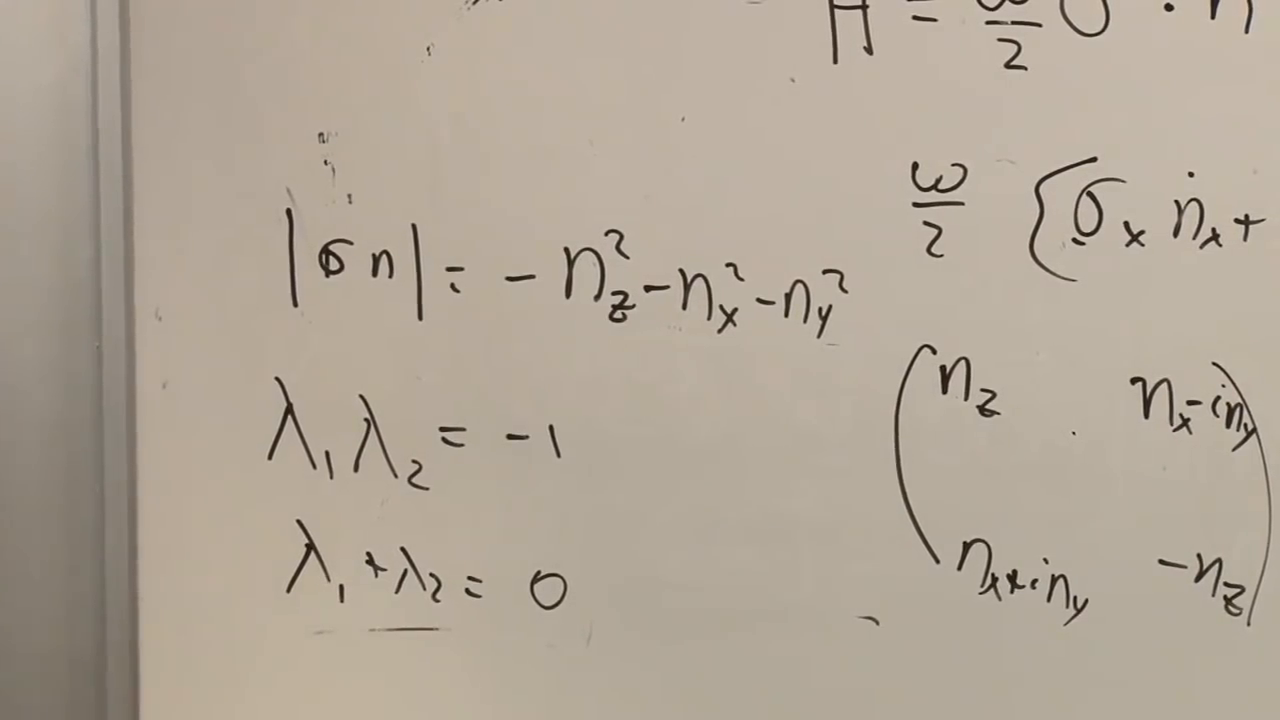
\includegraphics[width=0.86\textwidth]{lecture_05_figure_10.png}
\caption{トレースと行列式により、\(\bm\sigma\cdot\bm n\)の固有値は\(+1\)と\(-1\)に定まる。}
\lectureframe{01:59:20}
\end{figure}

したがって、
\begin{equation}
E_\pm=\pm\frac{\omega}{2},
\qquad
\Delta E=E_+-E_-=\omega.
\label{eq:l5-spin-gap}
\end{equation}
場の向きはエネルギーの固有ベクトルを変えるが、これら2つの固有値は変えない。

\begin{classroomqa}
\audiencequestion{光子放出はこれらの準位とどのように関係するのか。}
\lecturerresponse{放射場を含めると、高いスピン準位は現在の\(\hbar=1\)の規約でエネルギー\(\Delta E=\omega\)の光子を放出して低い準位へ崩壊しうる。そのときスピンは場の軸に沿った2つの反対向きの間で反転する。歳差運動の計算ではこの弱い放射結合を省いたので、スピンは放出する前に何度も歳差運動しうる。}
\end{classroomqa}

\begin{classroomqa}
\audiencequestion{なぜ磁場は量子演算子ではなく数として扱われるのか。}
\lecturerresponse{磁石は暫定的に、揺らぎと反跳が無視できる重い古典的装置として扱われる。完全な記述ではそれをより大きな量子系に含めるであろう。実用的な系と装置の分割は、装置が多くの自由度をもち、その関連変数の揺らぎが非常に小さいため電子がそれらを有意に変えられないときに正当化される。}
\end{classroomqa}

\begin{classroomqa}
\audiencequestion{滑らかな歳差運動の方程式は各々の個別の試行を記述するのか。}
\lecturerresponse{それらは期待値、したがって同一に準備された試行にわたる平均を記述する。個々の測定は確率的なままである。繰り返しのサンプルは理論的平均に近づく傾向があるが、確率論はすべての有限列に対して1つの厳密な結果を保証するものではない。ちょうど100万回の硬貨投げが正確に半分の表を含まなければならないわけではないのと同じである。}
\end{classroomqa}

\begin{classroomqa}
\audiencequestion{スピンが横向きを向いているなら、遷移は半分の光子を放出するのか。}
\lecturerresponse{いいえ。横向きのスピン状態は2つのエネルギー固有状態の重ね合わせである。対称な場合、それは上準位に2分の1の確率、下準位に2分の1の確率をもつ。したがってそれはエネルギー\(\omega\)の光子を1つ完全に放出するか、まったく放出しないかのいずれかでありうる。その平均放出エネルギーは\(\omega/2\)でありうるが、個々の光子が準位間隔の半分を運ぶことはない。}
\end{classroomqa}

これで単一スピンの非自明な時間に依存しない力学を使い尽くした。最初に不確定性を告げたのと同じ代数がその運動も生み出す。すなわち、非可換なパウリ行列がハミルトニアンを歳差運動に変え、ハミルトニアンと可換な成分は保存されたままである。次なる複雑さの増大は、別の1スピンのハミルトニアンではなく、独立な系を合成しもつれさせることができるより大きな状態空間である。
